%
% ---------------------------------------------------------------
% Copyright (C) 2012-2018 Gang Li
% ---------------------------------------------------------------
%
% This work is the default powerdot-tuliplab style test file and may be
% distributed and/or modified under the conditions of the LaTeX Project Public
% License, either version 1.3 of this license or (at your option) any later
% version. The latest version of this license is in
% http://www.latex-project.org/lppl.txt and version 1.3 or later is part of all
% distributions of LaTeX version 2003/12/01 or later.
%
% This work has the LPPL maintenance status "maintained".
%
% This Current Maintainer of this work is Gang Li.
%
%

\documentclass[
 size=14pt,
 paper=smartboard,  %a4paper, smartboard, screen
 mode=present, 		%present, handout, print
 display=slides, 	% slidesnotes, notes, slides
 style=tuliplab,  	% TULIP Lab style
 pauseslide,
 fleqn,leqno]{powerdot}


%我自己增加的两端对其用
\usepackage{ragged2e}
\renewcommand{\raggedright}{\leftskip=0pt \rightskip=0pt plus 0cm}


\usepackage{cancel}
\usepackage{caption}
\usepackage{stackengine}
\usepackage{smartdiagram}
\usepackage{attrib}
\usepackage{amssymb}
\usepackage{amsmath} 
\usepackage{amsthm} 
\usepackage{mathtools}
\usepackage{rotating}
\usepackage{graphicx}
\usepackage{boxedminipage}
\usepackage{rotate}
\usepackage{calc}
\usepackage[absolute]{textpos}
\usepackage{psfrag,overpic}
\usepackage{fouriernc}
\usepackage{pstricks,pst-3d,pst-grad,pstricks-add,pst-text,pst-node,pst-tree}
\usepackage{moreverb,epsfig,subfigure}
\usepackage{color}
\usepackage{booktabs}
\usepackage{etex}
\usepackage{breqn}
\usepackage{multirow}
\usepackage{natbib}
\usepackage{bibentry}
\usepackage{gitinfo2}
\usepackage{siunitx}
\usepackage{nicefrac}
%\usepackage{geometry}
%\geometry{verbose,letterpaper}
\usepackage{media9}
\usepackage{animate}
%\usepackage{movie15}
\usepackage{auto-pst-pdf}

%\usepackage{breakurl}
\usepackage{fontawesome}
\usepackage{xcolor}
\usepackage{multicol}



\usepackage{verbatim}
\usepackage[utf8]{inputenc}
\usepackage{dtk-logos}
\usepackage{tikz}
\usepackage{adigraph}
%\usepackage{tkz-graph}
\usepackage{hyperref}
%\usepackage{ulem}
\usepackage{pgfplots}
\usepackage{verbatim}
\usepackage{fontawesome}


\usepackage{todonotes}
% \usepackage{pst-rel-points}
\usepackage{animate}
\usepackage{fontawesome}

\usepackage{listings}
\lstset{frameround=fttt,
frame=trBL,
stringstyle=\ttfamily,
backgroundcolor=\color{yellow!20},
basicstyle=\footnotesize\ttfamily}
\lstnewenvironment{code}{
\lstset{frame=single,escapeinside=`',
backgroundcolor=\color{yellow!20},
basicstyle=\footnotesize\ttfamily}
}{}


\usepackage{hyperref}
\hypersetup{ % TODO: PDF meta Data
  pdftitle={Kaggle sildes},
  pdfauthor={Wang Mingxi},
  pdfpagemode={FullScreen},
  pdfborder={0 0 0}
}


% \usepackage{auto-pst-pdf}
% package to show source code

\definecolor{LightGray}{rgb}{0.9,0.9,0.9}
\newlength{\pixel}\setlength\pixel{0.000714285714\slidewidth}
\setlength{\TPHorizModule}{\slidewidth}
\setlength{\TPVertModule}{\slideheight}
\newcommand\highlight[1]{\fbox{#1}}
\newcommand\icite[1]{{\footnotesize [#1]}}

\newcommand\twotonebox[2]{\fcolorbox{pdcolor2}{pdcolor2}
{#1\vphantom{#2}}\fcolorbox{pdcolor2}{white}{#2\vphantom{#1}}}
\newcommand\twotoneboxo[2]{\fcolorbox{pdcolor2}{pdcolor2}
{#1}\fcolorbox{pdcolor2}{white}{#2}}
\newcommand\vpspace[1]{\vphantom{\vspace{#1}}}
\newcommand\hpspace[1]{\hphantom{\hspace{#1}}}
\newcommand\COMMENT[1]{}

\newcommand\placepos[3]{\hbox to\z@{\kern#1
        \raisebox{-#2}[\z@][\z@]{#3}\hss}\ignorespaces}

\renewcommand{\baselinestretch}{1.2}


\newcommand{\draftnote}[3]{
	\todo[author=#2,color=#1!30,size=\footnotesize]{\textsf{#3}}	}
% TODO: add yourself here:
%
\newcommand{\gangli}[1]{\draftnote{blue}{GLi:}{#1}}
\newcommand{\shaoni}[1]{\draftnote{green}{sn:}{#1}}
\newcommand{\gliMarker}
	{\todo[author=GLi,size=\tiny,inline,color=blue!40]
	{Gang Li has worked up to here.}}
\newcommand{\snMarker}
	{\todo[author=Sn,size=\tiny,inline,color=green!40]
	{Shaoni has worked up to here.}}

%%%%%%%%%%%%%%%%%%%%%%%%%%%%%%%%%%%%%%%%%%%%%%%%%%%%%%%%%%%%%%%%%%%%%%%%
% title
% TODO: Customize to your Own Title, Name, Address
%
\title{Summary Last Week - 2021.4.19}
\author{
Wang Mingxi
\\
\\Jilin University
\\College of Computer Science and Technology
}
\date{\gitCommitterDate}
%\date{\today} %暂时手写改动

% Customize the setting of slides
\pdsetup{
% TODO: Customize the left footer, and right footer
rf=\href{http://www.tulip.org.au}{
Last Changed by: \textsc{\gitCommitterName}\ \gitVtagn-\gitAbbrevHash\ (\gitAuthorDate)
%Last Changed by: \textsc{Bing Liu}\ \gitVtagn-\gitAbbrevHash\ (\today)
},
cf={flip00-kaggle},
}


\begin{document}

\maketitle

%\begin{slide}{Overview}
%\tableofcontents[content=sections]
%\end{slide}


%%==========================================================================================
%%
\begin{slide}[toc=,bm=]{Overview}
\tableofcontents[content=currentsection,type=1]
\end{slide}
%%
%%==========================================================================================


\section{Job summary}

%%==========================================================================================
%%
\begin{slide}{Git Project}

\begin{itemize}
\item The local repository is created on GitHub and three folders are created.
Local and remote repositories have also been synchronized. %So it is a little difficult for us.

\bigskip

\item Modified the text in the bottom right corner of the file by uploading the file to GitHub and then pulling it down.
\end{itemize}

\begin{center}
	\begin{figure}[htbp]
		
\includegraphics[scale=0.6]{./pic/kaka2.eps}
		\caption{The repository on GitHub}
	\end{figure}
\end{center}

\end{slide}
%%
%%==========================================================================================

%%==========================================================================================
%%
\begin{slide}{Notebook Amend}

\raggedright
I have read and studied one of XXX and have modified its contents.

\begin{center}
	\begin{figure}[htbp]
		\includegraphics[scale=0.3]{./pic/notebook.eps}
		\caption{The repository on GitHub}
	\end{figure}
\end{center}


\end{slide}
%%
%%==========================================================================================
\begin{slide}{Kaggle Subject}
%当有多个Kaggle Subject而只想在目录出现一次时,在后面几次Kaggle Subject前加上[toc=,bm=]
	\raggedright
	The San Francisco Crime Classification Forecast is a multi-classification problem that asks us to predict crime types.Given some characteristics, let the model predict the type of output crime based on the input.
	\begin{center}
		\begin{figure}[htbp]
			\includegraphics[scale=0.4]{./pic/SF.eps}
			\caption{The repository on GitHub}
		\end{figure}
	\end{center}

\end{slide}

\begin{slide}[toc=,bm=]{Kaggle Subject}
	\begin{itemize}
	\item The data analysis
	\end{itemize}
	\bigskip
	
	The data includes the time of the crime, the place of the crime, the description of the crime (in text form), the final disposition, the type of crime, etc.Crime data correlate with crime types.The function of the model is to analyze the data set to find out the relationship and carry out the classification and prediction of crime types.
	
\end{slide}

\begin{slide}[toc=,bm=]{Kaggle Subject}
	\begin{itemize}
	\item The data processing
	\end{itemize}
	\bigskip
	
	The daily features can be decomposed into more detailed contents to obtain more detailed features, thus improving the accuracy of the model.
	For example, the date is disassembled from a comprehensive form of adults, months, days, hours, minutes, etc
	What we found was that there was a difference in the type of crime that was committed inside the building and at the intersection.Findings like this suggest that there are characteristics that have a direct impact on the predicted outcome, as will be explained in more detail later.
\end{slide}

\begin{slide}[toc=,bm=]{Kaggle Subject}
	\begin{itemize}
		\item The data cleaning
	\end{itemize}
	\bigskip
	Some data needs to be cleaned up.There are duplicate elements in the data set, and those are the ones that we want to get rid of.In addition, in some obviously against the common sense of the wrong data, we also want to delete.For example, we find that there are crimes that we know are located in the ocean by latitude and longitude analysis, and those are the few crimes that we don't care about.
	\begin{center}
		\begin{figure}[htbp]
			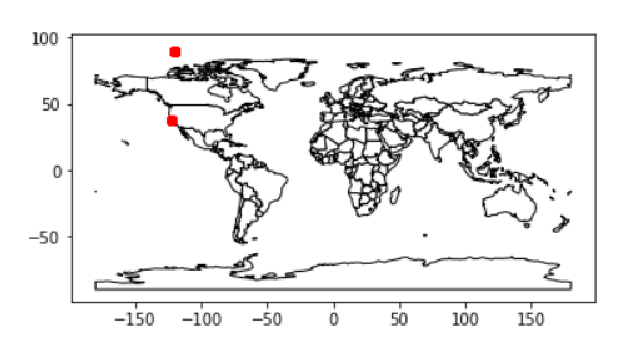
\includegraphics[scale=0.6]{./pic/cf_map.eps}
			\caption{The repository on GitHub}
		\end{figure}
	\end{center}	
	
\end{slide}

\begin{slide}[toc=,bm=]{Kaggle Subject}
	\begin{itemize}
		\item Build a model
	\end{itemize}
	\bigskip
	The decision tree was used to build the model. After 23 rounds of training, the model training was completed and the score on the test set was 2.3.However, there are still some unexplained errors and problems in the program operation. I will continue to modify them as soon as possible.
	
\end{slide}

\section{Next Week's Work}


\begin{slide}{Work arrangement}

I will modify the remaining notebook, and then complete the git repository.
Also the Kaggle topic related process to continue to improve, and modify the code related bugs, complete the coding work


\end{slide}
%%
%%==========================================================================================

%%==========================================================================================
%%
\begin{slide}{Thanks}

Thankes!

\end{slide}
%%
%%==========================================================================================

\section{Algorithm}
%\begin{slide}{Algorithm one}
%\includegraphics*[scale=0.2]{1.png}
%\end{slide}
\begin{slide}[toc=,bm=]{Algorithm}

\end{slide}

\section{Conclusion}
%%==========================================================================================
%%
\begin{slide}[toc=,bm=]{Conclusion}

\end{slide}
%\begin{slide}{Result}
%	\includegraphics*[scale=0.7]{result.png}
%\end{slide}

\begin{slide}[toc=,bm=]{Conclusion}



\end{slide}
%%
%%==========================================================================================


%%==========================================================================================
% TODO: Contact Page
\begin{wideslide}[toc=,bm=]{Contact Information}
\centering
\vspace{\stretch{1}}
\twocolumn[
lcolwidth=0.35\linewidth,
rcolwidth=0.65\linewidth
]
{
% \centerline{
\includegraphics[scale=.2]{tulip-logo.eps}}
}
{
\vspace{\stretch{1}}
Wang Mingxi\\
College of Computer Science and Technology\\
Jilin University, China
\begin{description}
 \item[\textcolor{orange}{\faEnvelope}] \href{mailto:bliu@tulip.academy}
 {\textsc{\footnotesize{bliu@tulip.academy}}}

 \item[\textcolor{orange}{\faHome}] \href{http://www.tulip.org.au}
 {\textsc{\footnotesize{Team for Universal Learning and Intelligent Processing}}}
\end{description}
}
\vspace{\stretch{1}}
\end{wideslide}

\end{document}

\endinput
